%Text Books : \cite{chartrand}
%Module 1 : Introduction to Graphs and Algorithms
%What is graph? The degree of a vertex, isomorphic graphs, subgraphs, degree sequences, connected graphs, cutvertices and blocks, special graphs, digraphs, algorithmic complexity, Search algorithms, sorting algorithms, greedy algorithms,, representing graphs in a computer.
%( Chapter 1 Sections 1.1 to 1.9, Chapter 2 Sections 2.1, 2.2 , 2.3, 2.5 and 2.6 of \cite{chartrand} ) (24 hours)
%Module 2 : Trees, paths and distances
%Properties of trees, rooted trees, Depth-first search, breadth-first search, the minimum spanning tree problem
%Distance in a graphs, distance in weighted graphs, the centre and median of a graph, Activity digraphs and critical paths.
%(Chapter 3 sections 3.1 to 3.3, 3.4 and 3.5 , Chapter 4 of \cite{chartrand} ) (22 hours)
%Module 3 : Networks
%An introduction to networks, the max-flow min-cut theorem, the max-flow min-cut algorithm, Connectivity and edge connectivity, Mengers theorem.
%( Chapter 5 sections 5.1 , 5.2 , 5.3 and 5.5 of \cite{chartrand} ) (22 hours)
%Module 4 : Matchings and Factorizations
%An introduction to matchings, maximum matchings in a bipartite graph, Factorizations, Block Designs.
%(Chapter 6 sections 6.1 , 6.2 , 6.4 and 6.5 of \cite{chartrand} ) (22 hours)

%Need to get a copy of this book !!
%List of Algorithms
%Module 1 - \cite{chartrand} 1, 2
%Module 2 - \cite{chartrand} 3, 4
%Module 3 - \cite{chartrand} 5
%Module 4 - \cite{chartrand} 6
%Missing - 7, 8?

%\chapter{An Introduction to Graphs}
\section{What is a Graph ?}
\begin{definition}[graph]
	A graph $G$ is a finite nonempty set $V(G)$ and a family $E(G)$ of 2-element subsets of $V(G)$.
\end{definition}

\begin{remark}
	Elements of $V(G)$ are called \textbf{vertices} and elements of $E(G)$ are called \textbf{edges} of the graph $G$.
	Suppose $\{u,v\}$ be an edge of a graph $G$. We may represent this edge by $uv$.\\

	Two vertices $u,v$ are \textbf{adjacent} if there exists an edge $e = uv$ joining them.
\end{remark}

\begin{definition}[multigraph]
	A graph with parallel edges is called a multigraph.
\end{definition}
\begin{definition}[psueudograph]
	A graph with parallel egdes and loops is called a psuedograph.
\end{definition}

\begin{definition}
	The number of vertices in graph $G$ is the order of the graph $G$.
	The number of edge in graph $G$ is the size of the graph $G$.
\end{definition}
\begin{remark}
	A graph $G$ of order $p$ and size $q$ is called a $(p,q)$ graph.
\end{remark}

\section{The Degree of a Vertex}
\begin{definition}[neighbourhood]
	Let $v$ be a vertex of graph $G$.
	The neighbourhood of $v$, $N(v)$ is the set of all vertices adjacent to it.
	$$ N(v) = \{ u \in V(G) : uv \in E(G) \} $$
\end{definition}
\begin{remark}
	The \textbf{degree} of a vertex $v$ is the cardinality of the neighbourhood of $v$ in graph $G$.
	$$ deg\ v = |N(v)| $$
	An edge of zero degree is called an \textbf{isolated vertex}.
	An edge of odd(even) degree is called an \textbf{odd(even) edge}.
\end{remark}

\begin{remark}
	Let $e=uv$ be an edge of a graph $G$.
	Then $e$ is \textbf{incident} on both $u$ and $v$.
\end{remark}

\begin{theorem}[First Theorem]
	Let $G$ be a graph of order $p$ and size $q$ with vertex set $V(G) = \{ v_1,v_2,\dots,v_p \}$.
	Then,
	$$ \sum_{i=1}^p deg\ v_i = 2q $$
\end{theorem}
\begin{proof}
	Since degrees of vertices are counted, every edge is counted twice (from both ends). Thus the sum of degrees is twice the size of the graph.
\end{proof}

\begin{corollary}
	Every graph has even number of odd vertices.
\end{corollary}
\begin{proof}
	By first theorem of graph theory, the sum of degree is an even integer.
	Suppose there are odd number of odd vertices.
	Then the sum of degrees is odd which is a contradiction.
	Therefore, there are even number of odd vertices in any graph $G$.
\end{proof}

\begin{definition}[regular]
	A graph $G$ is $r$-regular if every vertex of $G$ has degree $r$.
\end{definition}

\begin{definition}[complement]
	Let $G$ be a graph. The complement $\bar{G}$ is the graph with vertex set $V(G) = V(\bar{G})$ and $uv$ is an edge of $\bar{G}$ if $uv$ is not an edge of $G$.
\end{definition}

\section*{Problem Set 1.2}
\begin{enumerate}
	\item Prove that every graph of order $n \ge 2$ has at least two vertices of the same degree.
	\begin{proof}
		Let $G$ be a graph of order $p$. Suppose every vertex is of different degree. Then there exists a vertex of degree $0$ and a vertex of degree $p-1$. This is a contradiction as the vertex of degree $0$ is not adjacent to any other vertex and the vertex of degree $p-1$ is adjacent to every other vertex.
	\end{proof}
		\setcounter{enumi}{6}
	\item
	\begin{enumerate}
	\item Construct an $r$-regular graph of order $8$ for each $r$, $0 \le r < 8$.\\
		(See Figure \ref{dia:regularOrder8})
	\begin{figure}[hbt]
	\centering
	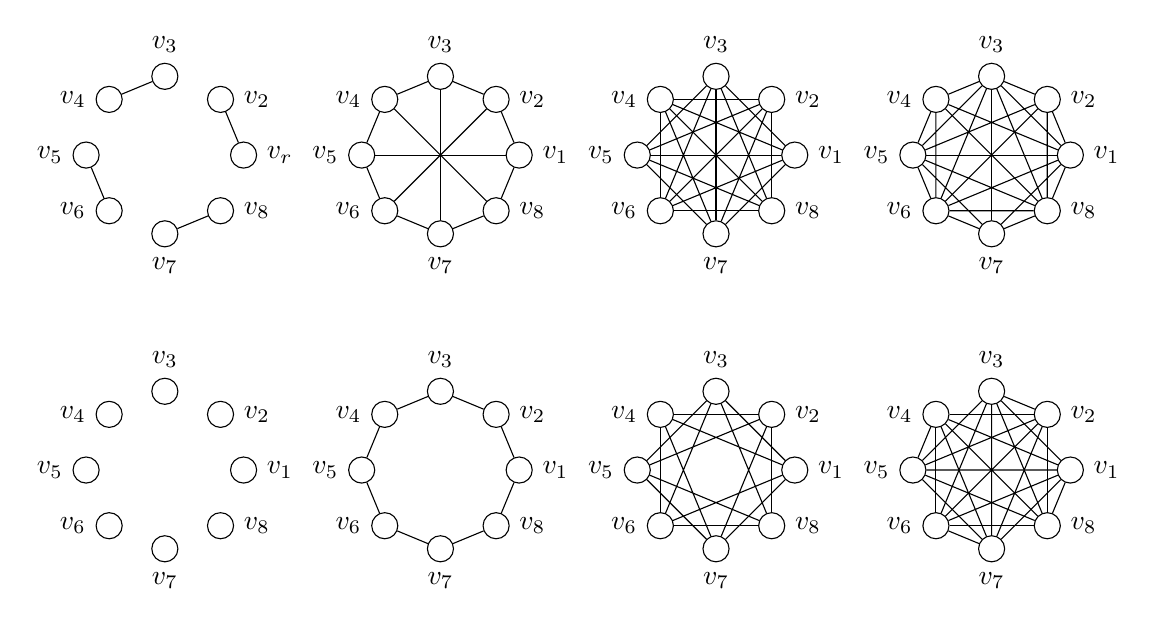
\begin{tikzpicture}[scale=0.5]
		\draw (0,0) node (a)[circle]{};
		\draw (a) ++(0:2) node (a1)[draw,circle,label=right:$v_1$]{};
		\draw (a) ++(45:2) node (a2)[draw,circle,label=right:$v_2$]{};
		\draw (a) ++(90:2) node (a3)[draw,circle,label=above:$v_3$]{};
		\draw (a) ++(135:2) node (a4)[draw,circle,label=left:$v_4$]{};
		\draw (a) ++(180:2) node (a5)[draw,circle,label=left:$v_5$]{};
		\draw (a) ++(225:2) node (a6)[draw,circle,label=left:$v_6$]{};
		\draw (a) ++(-90:2) node (a7)[draw,circle,label=below:$v_7$]{};
		\draw (a) ++(-45:2) node (a8)[draw,circle,label=right:$v_8$]{};

		\draw (0,8) node (b)[circle]{};
		\draw (b) ++(0:2) node (b1)[draw,circle,label=right:$v_r$]{};
		\draw (b) ++(45:2) node (b2)[draw,circle,label=right:$v_2$]{};
		\draw (b) ++(90:2) node (b3)[draw,circle,label=above:$v_3$]{};
		\draw (b) ++(135:2) node (b4)[draw,circle,label=left:$v_4$]{};
		\draw (b) ++(180:2) node (b5)[draw,circle,label=left:$v_5$]{};
		\draw (b) ++(225:2) node (b6)[draw,circle,label=left:$v_6$]{};
		\draw (b) ++(-90:2) node (b7)[draw,circle,label=below:$v_7$]{};
		\draw (b) ++(-45:2) node (b8)[draw,circle,label=right:$v_8$]{};
		\draw (b1)--(b2);
		\draw (b3)--(b4);
		\draw (b5)--(b6);
		\draw (b7)--(b8);

		\draw (7,0) node (c)[circle]{};
		\draw (c) ++(0:2) node (c1)[draw,circle,label=right:$v_1$]{};
		\draw (c) ++(45:2) node (c2)[draw,circle,label=right:$v_2$]{};
		\draw (c) ++(90:2) node (c3)[draw,circle,label=above:$v_3$]{};
		\draw (c) ++(135:2) node (c4)[draw,circle,label=left:$v_4$]{};
		\draw (c) ++(180:2) node (c5)[draw,circle,label=left:$v_5$]{};
		\draw (c) ++(225:2) node (c6)[draw,circle,label=left:$v_6$]{};
		\draw (c) ++(-90:2) node (c7)[draw,circle,label=below:$v_7$]{};
		\draw (c) ++(-45:2) node (c8)[draw,circle,label=right:$v_8$]{};
		\draw (c1)--(c2)--(c3)--(c4)--(c5)--(c6)--(c7)--(c8)--(c1);

		\draw (7,8) node (d)[circle]{};
		\draw (d) ++(0:2) node (d1)[draw,circle,label=right:$v_1$]{};
		\draw (d) ++(45:2) node (d2)[draw,circle,label=right:$v_2$]{};
		\draw (d) ++(90:2) node (d3)[draw,circle,label=above:$v_3$]{};
		\draw (d) ++(135:2) node (d4)[draw,circle,label=left:$v_4$]{};
		\draw (d) ++(180:2) node (d5)[draw,circle,label=left:$v_5$]{};
		\draw (d) ++(225:2) node (d6)[draw,circle,label=left:$v_6$]{};
		\draw (d) ++(-90:2) node (d7)[draw,circle,label=below:$v_7$]{};
		\draw (d) ++(-45:2) node (d8)[draw,circle,label=right:$v_8$]{};
		\draw (d1)--(d2)--(d3)--(d4)--(d5)--(d6)--(d7)--(d8)--(d1);
		\draw (d1)--(d5);
		\draw (d2)--(d6);
		\draw (d3)--(d7);
		\draw (d4)--(d8);

		\draw (14,0) node (e)[circle]{};
		\draw (e) ++(0:2) node (e1)[draw,circle,label=right:$v_1$]{};
		\draw (e) ++(45:2) node (e2)[draw,circle,label=right:$v_2$]{};
		\draw (e) ++(90:2) node (e3)[draw,circle,label=above:$v_3$]{};
		\draw (e) ++(135:2) node (e4)[draw,circle,label=left:$v_4$]{};
		\draw (e) ++(180:2) node (e5)[draw,circle,label=left:$v_5$]{};
		\draw (e) ++(225:2) node (e6)[draw,circle,label=left:$v_6$]{};
		\draw (e) ++(-90:2) node (e7)[draw,circle,label=below:$v_7$]{};
		\draw (e) ++(-45:2) node (e8)[draw,circle,label=right:$v_8$]{};
		%\draw (e1)--(e2)--(e3)--(e4)--(e5)--(e6)--(e7)--(e8)--(e1);
		\draw (e1)--(e3)--(e5)--(e7)--(e1);
		\draw (e2)--(e4)--(e6)--(e8)--(e2);
		\draw (e1)--(e4)--(e7)--(e2)--(e5)--(e8)--(e3)--(e6)--(e1);

		\draw (14,8) node (f)[circle]{};
		\draw (f) ++(0:2) node (f1)[draw,circle,label=right:$v_1$]{};
		\draw (f) ++(45:2) node (f2)[draw,circle,label=right:$v_2$]{};
		\draw (f) ++(90:2) node (f3)[draw,circle,label=above:$v_3$]{};
		\draw (f) ++(135:2) node (f4)[draw,circle,label=left:$v_4$]{};
		\draw (f) ++(180:2) node (f5)[draw,circle,label=left:$v_5$]{};
		\draw (f) ++(225:2) node (f6)[draw,circle,label=left:$v_6$]{};
		\draw (f) ++(-90:2) node (f7)[draw,circle,label=below:$v_7$]{};
		\draw (f) ++(-45:2) node (f8)[draw,circle,label=right:$v_8$]{};
		\draw (f1)--(f3)--(f5)--(f7)--(f1);
		\draw (f2)--(f4)--(f6)--(f8)--(f2);
		\draw (f1)--(f4)--(f7)--(f2)--(f5)--(f8)--(f3)--(f6)--(f1);
		\draw (f1)--(f5);
		\draw (f2)--(f6);
		\draw (f3)--(f7);
		\draw (f4)--(f8);

		\draw (21,0) node (g)[circle]{};
		\draw (g) ++(0:2) node (g1)[draw,circle,label=right:$v_1$]{};
		\draw (g) ++(45:2) node (g2)[draw,circle,label=right:$v_2$]{};
		\draw (g) ++(90:2) node (g3)[draw,circle,label=above:$v_3$]{};
		\draw (g) ++(135:2) node (g4)[draw,circle,label=left:$v_4$]{};
		\draw (g) ++(180:2) node (g5)[draw,circle,label=left:$v_5$]{};
		\draw (g) ++(225:2) node (g6)[draw,circle,label=left:$v_6$]{};
		\draw (g) ++(-90:2) node (g7)[draw,circle,label=below:$v_7$]{};
		\draw (g) ++(-45:2) node (g8)[draw,circle,label=right:$v_8$]{};
		\draw (g1)--(g3)--(g5)--(g7)--(g1);
		\draw (g2)--(g4)--(g6)--(g8)--(g2);
		\draw (g1)--(g4)--(g7)--(g2)--(g5)--(g8)--(g3)--(g6)--(g1);
		\draw (g1)--(g5)--(g4)--(g8)--(g1);
		\draw (g2)--(g3)--(g7)--(g6)--(g2);

		\draw (21,8) node (h)[circle]{};
		\draw (h) ++(0:2) node (h1)[draw,circle,label=right:$v_1$]{};
		\draw (h) ++(45:2) node (h2)[draw,circle,label=right:$v_2$]{};
		\draw (h) ++(90:2) node (h3)[draw,circle,label=above:$v_3$]{};
		\draw (h) ++(135:2) node (h4)[draw,circle,label=left:$v_4$]{};
		\draw (h) ++(180:2) node (h5)[draw,circle,label=left:$v_5$]{};
		\draw (h) ++(225:2) node (h6)[draw,circle,label=left:$v_6$]{};
		\draw (h) ++(-90:2) node (h7)[draw,circle,label=below:$v_7$]{};
		\draw (h) ++(-45:2) node (h8)[draw,circle,label=right:$v_8$]{};
		\draw (h1)--(h2)--(h3)--(h4)--(h5)--(h6)--(h7)--(h8)--(h1);
		\draw (h1)--(h3)--(h5)--(h7)--(h1)--(h4)--(h6)--(h8)--(h2)--(h5)--(h8)--(h3)--(h6)--(h1);
		\draw (h1)--(h5);
		\draw (h2)--(h6);
		\draw (h3)--(h7);
		\draw (h4)--(h8);
	\end{tikzpicture}
	\caption{$r$-regular graph of order $8$}
	\label{dia:regularOrder8}
	\end{figure}
\item Determine the complement of each graph constructed in (a).\\
	(complements are already there in the list)
	\item Prove that if $G$ is a regular graph. Then $\bar{G}$ is regular.
	\begin{proof}
	Let $G$ be an $r$-regular graph of order $p$. Let $v \in V(G)$. Then $deg\ v = r$. Thus, there are $r$ vertices adjacent to $v$ in graph $G$. In other words, there are $p-r-1$ vertices non-adjacent to $v$ in $G$. Therefore, $deg\ v$ is the complement graph $\bar{G}$ is $p-r-1$. Since $v \in V(G)$ is arbitrary, $\bar{G}$ is $p-r-1$-regular graph.
	\end{proof}
\end{enumerate}
\end{enumerate}

\section{Isomorphic Graphs}
\begin{definition}[isomorphism]
	Two graphs $G_1,G_2$ are isomorphic if there exists a bijection $$\phi : V(G_1) \to V(G_2) \text{ such that }uv \in E(G_1) \iff \phi(u)\phi(v) \in E(G_2)$$
\end{definition}
\begin{remark}
	Two graphs $G_1,G_2$ are equal if $V(G_1) = V(G_2)$ and $E(G_1) = E(G_2)$. Clearly, equal graphs are isomorphic. However, isomorphic graphs are not equal.
\end{remark}

\subsection*{Problem Set 1.3}
\begin{enumerate}
	\item Find two non-isomorphic $3$-regualr graphs of order $6$ and size $9$.\\
		There are exactly two non-isomorphic $3$-regular graphs of order $6$. By first theorem of graph theory, the size of such a graph is always $9$.(see Figure \ref{dia:3r6o}.
	\begin{figure}[hbt]
		\centering
		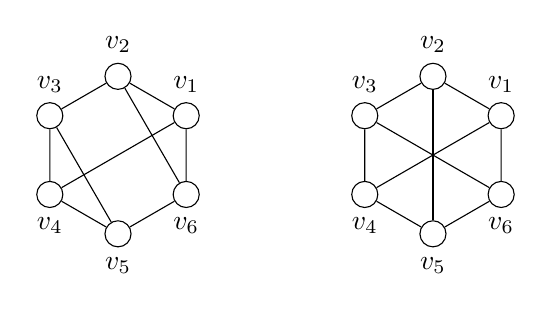
\begin{tikzpicture}[scale=0.5]
			\draw (8,0) node (v){};
			\draw (v) ++(30:2) node (v1)[draw,circle,label=above:$v_1$]{};
			\draw (v) ++(90:2) node (v2)[draw,circle,label=above:$v_2$]{};
			\draw (v) ++(150:2) node (v3)[draw,circle,label=above:$v_3$]{};
			\draw (v) ++(-150:2) node (v4)[draw,circle,label=below:$v_4$]{};
			\draw (v) ++(-90:2) node (v5)[draw,circle,label=below:$v_5$]{};
			\draw (v) ++(-30:2) node (v6)[draw,circle,label=below:$v_6$]{};
			\draw (v1)--(v2)--(v3)--(v4)--(v5)--(v6)--(v1);
			\draw (v1)--(v4);
			\draw (v2)--(v5);
			\draw (v3)--(v6);

			\draw (0,0) node (u){};
			\draw (u) ++(30:2) node (u1)[draw,circle,label=above:$v_1$]{};
			\draw (u) ++(90:2) node (u2)[draw,circle,label=above:$v_2$]{};
			\draw (u) ++(150:2) node (u3)[draw,circle,label=above:$v_3$]{};
			\draw (u) ++(-150:2) node (u4)[draw,circle,label=below:$v_4$]{};
			\draw (u) ++(-90:2) node (u5)[draw,circle,label=below:$v_5$]{};
			\draw (u) ++(-30:2) node (u6)[draw,circle,label=below:$v_6$]{};
			\draw (u1)--(u2)--(u3)--(u4)--(u5)--(u6)--(u1);
			\draw (u1)--(u4);
			\draw (u2)--(u6);
			\draw (u3)--(u5);
		\end{tikzpicture}
		\caption{$3$-regular graph of order $6$}
		\label{dia:3r6o}
	\end{figure}
	\item
	\begin{enumerate}
	\item Draw all eleven nonisomorphic graphs of order $4$\\
		$P_4,C_4,\bar{C_4},K_4,\bar{K_4},K_4-e,K_2+2K_1,K_{1,3},\bar{K}_{1,3},P_2+K_1,C_3+e$
	\item Let $S$ be a set of $23$ graphs of order $4$, then $S$ has at least three graphs that are pairwise isomorphic.
	\begin{proof}
		There are at most eleven non-isomorphic graphs of order $r$.
		By pigeonhole principle, in a family of $23$ graphs of order $4$ at least three graphs are pairwise isomorphic.
	\end{proof}
	\end{enumerate}
	\item Give an example of a graph $G$ of order $5$ such that $G \cong \bar{G}$.\\
		There are only two such graphs upto isomorphism.(see Figure \ref{dia:sc5})
	\begin{figure}[hbt]
	\centering
	\begin{tikzpicture}
		\draw (0,0) node (u){};
		\draw (u) ++(36:2) node (u1)[draw,circle,label=right:$v_1$]{};
		\draw (u) ++(108:2) node (u2)[draw,circle,label=above:$v_2$]{};
		\draw (u) ++(180:2) node (u3)[draw,circle,label=left:$v_3$]{};
		\draw (u) ++(-108:2) node (u4)[draw,circle,label=above:$v_4$]{};
		\draw (u) ++(-36:2) node (u5)[draw,circle,label=right:$v_5$]{};
		\draw (u1)--(u2)--(u3)--(u4)--(u5);
		\draw (u2)--(u4);

		\draw (6,0) node (v){};
		\draw (v) ++(36:2) node (v1)[draw,circle,label=right:$v_1$]{};
		\draw (v) ++(108:2) node (v2)[draw,circle,label=above:$v_2$]{};
		\draw (v) ++(180:2) node (v3)[draw,circle,label=left:$v_3$]{};
		\draw (v) ++(-108:2) node (v4)[draw,circle,label=above:$v_4$]{};
		\draw (v) ++(-36:2) node (v5)[draw,circle,label=right:$v_5$]{};
		\draw (v1)--(v2)--(v3)--(v4)--(v5)--(v1);
	\end{tikzpicture}
	\caption{Self-complementary graphs of order $5$}
	\label{dia:sc5}
	\end{figure}
	\item There are three regular graphs of order $5$, and eight regular graphs of order $6$. Draw all of them\\
		Three regular graphs of order $5$ are $C_5,K_5$ and $\bar{K}_5$.\\
		Eight regular graphs of order $6$ are $3K_2,C_6,2K_3,K_6$ and complements.
	\item Prove that two graph $G_1$ and $G_2$ are isomorphic if and only if their complements are isomorphic.
	\begin{proof}
	\begin{align*}
	G_1 \cong G_2 
		& \iff \phi : G_1 \to G_2,\ \left[uv \in E(G_1) \iff  \phi(u)\phi(v) \in E(G_2)\right] \\
		& \iff \phi : G_1 \to G_2,\ \left[uv \notin E(G_1) \iff \phi(u)\phi(v) \notin E(G_2)\right] \\
		& \iff \bar{G}_1 \cong \bar{G}_2
	\end{align*}
	\end{proof}
	\item Draw all nonisomorphic $4$-regular graphs of order $7$.\\
		There are only two distinct $2$-regular graphs of order $7$ upto isomorphism. The graphs are $C_7$ and $C_3+C_4$. Every $4$-regular graphs of order $7$ is complement of some $2$-regular graph of order $7$. Thus there are only two $4$-regular graphs of order $7$. The graphs are $\bar{C}_7$ and $\overline{C_3+C_4}$.

\begin{commentary}
	There are two trivial regular graphs $K_p$ and $\bar{K}_p$. In order to count regular graphs of order $p$, it is always easier to count $r$-regular graphs for $0 \le r \le \lfloor (p-1)/2 \rfloor$.\\

	For example, $p=8$. We need to construct all nonisomorphic $r$-regular graphs of order $8$ for $r=0,1,2,3$. There are one graph each for $r=0,1$. The $2$-regular graphs are always disjoint union of cycles. Thus, the only possibilities are $C_3+C_5, 2C_4$ and $C_8$. Finding $3$-regular graphs of order $8$ is the hard part.\\

	You may find various classifications of all small graphs (upto order $13$) at \href{https://www.graphclasses.org/smallgraphs.html}{graphclasses.org}. And there is a combinatorial result on number of regular graphs of order $p$ available at \href{https://oeis.org/A051031}{oeis.org}.\\

	As per OEIS there are six nonisomorphic $3$ regular graph of order $8$. Thus, there are twenty two nonisomophic regular graphs of order $8$.
\end{commentary}
	\setcounter{enumi}{8}
	\item Show that the relation `is isomorphic to' is an equivalence relation on the set of all graphs.
	\begin{proof}
		Trivially $G \cong G$ as $G$ is equal to itself and equal graphs are always isomorphic.\\

		Suppose $G_1 \cong G_2$. Then there exists a bijection $\phi : V(G_1) \to V(G_2)$ such that $uv \in E(G_1) \iff \phi(u)\phi(v) \in E(G_2)$. Clearly, $\phi^{-1} : V(G_2) \to V(G_1)$ is an isomorphism. Thus, $G_2 \cong G_1$.\\

		Suppose $G_1 \cong G_2$ and $G_2 \cong G_3$.
		Then there exist bijection $\phi : V(G_1) \to V(G_2)$ such that $uv \in E(G_1) \iff \phi(u)\phi(v) \in E(G_2)$ and bijection $\psi : V(G_2) \to V(G_3)$ such that
		$$\phi(u)\phi(v) \in E(G_2) \iff \psi(\phi(u))\psi(\phi(v)) \in E(G_3)$$
		Clearly, $\psi \circ \phi : V(G_1) \to V(G_3)$ is a bijection such that
		$$ uv \in E(G_1) \iff \psi \circ \phi(u) \psi\circ\phi(v) \in E(G_3) $$
		Therefore, $G_1 \cong G_3$.
	\end{proof}
\end{enumerate}
\section{Subgraphs}
---to continue-- (pp. 12)
\section{Degree Sequences}
\section{Connected Graphs}
\section{Cut-Vertices and Bridges}
\section{Special Graphs}
\section{Digraphs}

%\chapter{An Introduction to Algorithms}
\section{Algorithmic Complexity}
\section{Serach Algorithms}
\section{Sorting Algorithms}
%\section{Introducing NP-Completeness*}
\setcounter{section}{4}
\section{Greedy Algorithms}
\section{Representing Graphs in a Computer}

%Module 2
%\chapter{Trees}
\section{Properties of Trees}
\section{Rooted Trees}
\section{Depth-First Search}
\section{Depth-First Search : A Tool for Finding Blocks}
\section{Breadth-First Search}
\section{The Minimum Spanning Tree Problem}

%\chapter{Paths and Distance in Graphs}
\section{Distance in Graphs}
\section{Distance in Weighted Graphs}
\section{The Center and Median of a Graph}
\section{Activity Digraphs and Critical Paths}
%\section{Error Correcting Codes$^\ast$}

%Module 3
\section{Networks}
\subsection{An Introduction to Networks}
\begin{definition}
	A \textbf{network} $N$ is a digraph $D$ with two special vertices source $s$ and sink $t$ together with a capacity function $c : E(D) \to \mathbb{Z}$ such that for every arc $a = (u,v)$ of the digraph, $c(u,v)$ is non-negative.
\end{definition}

\begin{remark} Mathematical Modeling using Network,
	\begin{enumerate}
		\item There is no restriction on indegree/outdegree of source/sink vertices of the digraph $D$ of a network $N$.
		\item Applications of Network : Transportation problem.
	\end{enumerate}
\end{remark}

\begin{description}
	\item[$c(u,v)$] is the capacity of the arc $(u,v)$ of $D$
	\item[$N^+(x)$] $= \{ y \in V(D) : (x,y) \in E(D)\}$ is the out-neighbourhood of $x$.
	\item[$N^-(x)$] $= \{ y \in V(D) : (y,x) \in E(D)\}$ is the in-neighbourhood of $x$.
\end{description}

\begin{definition}
	A \textbf{flow f in a network N} is function $f : E(D) \to \mathbb{Z}$ such that
	\begin{enumerate*}
		\item each edge satisfies capacity constraint and
		\item each vertex except source and sink satisfies conservation equation.
	\end{enumerate*}
\end{definition}

\begin{description}
	\item[capacity constraint] 
		\begin{equation}
		0 \le f(a) \le c(a) \text{ for every arc }a \in V(D)
		\end{equation}
	\item[conservation equation] 
		\begin{equation}
			\sum_{y \in N^+(x)} f(x,y) = \sum_{y \in N^-(x)} f(y,x),\ \forall \text{vertex } x \in V(D)-\{s,t\}
		\label{equ:conservation}
		\end{equation}
	\item[net flow out of $x$]
		\[ \sum_{y \in N^+(x)} f(x,y) - \sum_{y \in N^-(x)} f(y,x) \]
	\item[net flow into $x$]
		\[ \sum_{y \in N^-(x)} f(y,x) - \sum_{y \in N^+(x)} f(x,y) \]
\end{description}

\begin{definition}
	The \textbf{flow f in a network N} is the net flow out of source $s$.
\end{definition}

\begin{remark}
	\begin{enumerate}
		\item net flow out of/into $x \in V(D)-\{s,t\}$ is zero.
		\item Without loss of generality\footnote{If underlying digraph of a network is symmetric, then by replacing an arc $(u,v)$ with a new vertex $w$ and two arcs $(u,w),(w,v)$ gives an assymetric digraph.\cite{chartrand}pp.131}, underlying digraph is always assymetric.
	\end{enumerate}
\end{remark}

\begin{description}
	\item[$(X,Y)$] $=\{ (x,y) \in E(D) : x \in X,\ y \in Y \}$.\\
		Let $X,Y$ be non-empty subsets of $V(D)$ such that $X,Y$ are disjoint.
		Then $(X,Y)$ is the set of all arcs from $X$ to $Y$.
	\item[flow from $X$ to $Y$] is the sum of flow on each arc in $(X,Y)$
		\begin{equation}
		f(X,Y) = \sum_{(x,y) \in (X,Y)} f(x,y)
		\end{equation}
	\item[capacity of the partition $(X,Y)$] is the total capacity of arcs in $(X,Y)$
		\begin{equation}
		c(X,Y) = \sum_{(x,y) \in (X,Y)} c(x,y)
		\end{equation}
	\item[cut] Let $P \subset V(D)$ such that $s \in P$ and $t \notin P$ and $\bar{P} = V(D)-P$, then $(P,\bar{P})$ is a cut.
	\item[flow from $P$ to $\bar{P}$] is the sum of flow on each arc in $(P,\bar{P})$.
		\begin{equation}
		f(P,\bar{P}) = \sum_{(x,y) \in (P,\bar{P})} f(x,y)
		\end{equation}
	\item[flow from $\bar{P}$ to $P$] is the sum of flow on each arc in $(\bar{P},P)$
		\begin{equation}
		f(\bar{P},P) = \sum_{(x,y) \in (\bar{P},P)} f(x,y)
		\end{equation}
	\item[capacity of the cut $(P,\bar{P})$] is the total capacity of the arcs in $(P,\bar{P})$
		\begin{equation}
		c(P,\bar{P}) = \sum_{(x,y) \in (P,\bar{P})} c(x,y)
		\end{equation}
\end{description}

\begin{theorem}
	For any cut $(P,\bar{P})$, the flow in $N$ is $f(N) = f(P,\bar{P}) - f(\bar{P},P)$.
\end{theorem}
\begin{synopsis}
	The net flow out of source $s$ is the flow $f(N)$ in the network $N$.
	Let $(P,\bar{P})$ be a cut of $N$, then $s \in P$ and $t \notin P$.
	Suppose $P = \{ s\}$, then the theorem is true.
	Suppose $P$ is not singleton, then for each vertex $x \in P,\ x \ne s$, the net flow out of $x$ is zero by flow conservation equation.
	And flow between vertices in $P$ cancels out each other.
	Thus adding net flow out of each vertex in $P$, will be same as the net flow out of source which is the flow in the network, $f(N)$.
\end{synopsis}
\begin{proof}
	\begin{equation}
		\text{Flow, }f = \sum_{y \in N^+(s)} f(s,y) - \sum_{y \in N^-(s)} f(y,s)
	\end{equation}
	By conservation equation, we have $\forall x \in P,\ x \ne s$,
	\begin{equation}
		\sum_{y \in N^+(x)} f(x,y) - \sum_{y \in N^-(x)} f(y,x) = 0
	\end{equation}
	By above equations,
	\begin{align}
		\text{Flow, } f & = \sum_{x \in P} \sum_{y \in N^+(x)} f(x,y) - \sum_{x \in P} \sum_{y \in N^-(x)} f(y,x) \nonumber\\
				& = \sum_{(x,y) \in (P,\bar{P})} f(x,y) - \sum_{(y,x) \in (\bar{P},P)} f(y,x) 
	\end{align}
\end{proof}

\begin{corollary}
	Flow cannot exceed the capacity of any cut $(P,\bar{P})$.
	Further, $f(N) \le \min c(P,\bar{P})$.
\end{corollary}
\begin{synopsis}
	Let $(P,\bar{P})$ be a cut in network $N$, then by theorem the flow $f(N) =$  flow from $P$ to $\bar{P}$ - flow from $\bar{P}$ to $P$.
	Since the flow from $\bar{P}$ to $P$ is non-negative, $f(N) \le$ flow from $P$ to $\bar{P}$.
	Clearly, $f(x,y) \le c(x,y)$ by the capacity constaint.
	Thus $f(N) \le f(P,\bar{P}) \le c(P,\bar{P}) \le \min c(P,\bar{P})$.
\end{synopsis}
\begin{proof}
	\begin{align*}
		f(N) 	& = \sum_{(x,y) \in (P,\bar{P})} f(x,y) - \sum_{(y,x) \in (\bar{P},P)} f(y,x) \\
			& \le \sum_{(x,y) \in (P,\bar{P})} f(x,y) = f(P,\bar{P})\\ 
			& \le \sum_{(x,y) \in (P,\bar{P})} c(x,y) = c(P,\bar{P}),\quad \because \forall x,y \in V(D),\ f(x,y) \le c(x,y) \\
			& \le \min c(P,\bar{P})
	\end{align*}
\end{proof}

\begin{corollary}
	In a network $N$ flow is the net flow into the sink of $N$.
\end{corollary}
\begin{synopsis}
	Let $\bar{P} = \{ t \}$, then by theorem $f(N)$ is the net flow into the sink.
\end{synopsis}
\begin{proof}
	Suppose $P = V(D)-\{t\}$.
	Then by theorem, we have
	\begin{align*}
		f(N) 	& = \sum_{(x,y) \in (P,\bar{P})} f(x,y) - \sum_{(y,x) \in (\bar{P},P)} f(y,x) \\
			& = \sum_{x \in N^-(t)} f(x,t) - \sum_{x \in N^+(t)} f(t,x)
	\end{align*}
\end{proof}

\begin{remark}Exercise 5.1
	\begin{enumerate}
		\setcounter{enumi}{3}
		\item Let $N$ be a network with underlying digraph $D$ which has a vertex $v \in V(D) - \{ s,t \}$ with zero indegree.
			Clearly the flow into $v$ is zero.
			Thus flow out of $v$ is also zero by flow conservation equation.
			Let $N'$ be the network obtained from $N$ by deleting the vertex $v$.
			Then $f(N) = f(N')$.
	\end{enumerate}
\end{remark}

\subsection{The Max-Flow Min-Cut Theorem}
\begin{description}
	\item[maximum flow] A flow $f$ in network $N$ is maximum flow in $N$, if $f(N) \ge f'(N)$ for each flow $f'$ in $N$.
	\item[minimum cut] A cut $(P,\bar{P})$ in network $N$ is minimum cut of $N$,\\ if $c(P,\bar{P}) \le c(X,\bar{X})$ for each cut $(X,\bar{X})$ in $N$.
	\item[$f$-unsaturated] Let $f$ be a flow in network $N$ with underlying digraph $D$, and $Q = u_0,a_1,u_1,a_2,\cdots,u_{n-1},a_n,u_n$ be a semipath in $D$ such that every forward arc $a_i = (u_{i-1},u_i)$ has flow not upto its capacity, $f(a_i) < c(a_i)$ and every reverse arc $a_i = (u_i,u_{i-1})$ has some positive flow in it, $f(a_i) > 0$
	\item[f-augmenting semipath] Let $f$ be a flow in a network $N$ with underlying digraph $D$.
		Suppose semipath $Q = s,a_1,u_1,a_2,\cdots,u_{n-1},a_n,t$ (from source to sink) is $f$-unsaturated, then $Q$ is an $f$-augmenting semipath.
\end{description}

\begin{theorem}
	Let $f$ be a flow in a network $N$ with underlying digraph $D$.
	The flow $f$ is maximum in $N$ iff there is no $f$-augmenting semipath in $D$.
\end{theorem}
\begin{synopsis}
	Suppose $Q$ is an $f$-augmenting semipath in $D$, then there exists a flow $f^*$ in $N$ such that $f(N)+\Delta = f^*(N)$.
	Therefore, $f$ is not a maximum flow in $N$.
	Suppose there is no $f$-augmenting semipath in $D$, then there exists a cut $(P,\bar{P})$ such that $f(a) = c(a)\ \forall a \in (P,\bar{P})$ and $f(a) = 0\ \forall a \in (\bar{P},P)$.
	Suppose $f^*$ in a maximum flow in $N$, then $f(N) \le f^*(N) \le c(P,\bar{P}) = f(N)$.
\end{synopsis}
\begin{proof}
	Let $f$ be a flow in a network $N$ with underlying digraph $D$ and $Q = s, a_1, u_1, a_2, u_2, \cdots, u_{n-1}, a_n, t$ be an $f$-augmenting semipath in $D$.
	\[\text{define } \Delta_i = \begin{cases}
		c(a_i) - f(a_i) \text{ for every forward arc } a_i \in Q, \\
		f(a_i) \text{ for every reverse arc } a_i \in Q,
	\end{cases} \]
	Define $\Delta = \min \{ \Delta_i \}$.
	Also define $f^* : E(D) \to \mathbb{Z}$ such that 
	\[ f^*(a_i) = \begin{cases} f(a) + \Delta \text{, for every forward arc } a_i \in Q, \\
	f(a) - \Delta \text{, for every reverse arc } a_i \in Q, \\
	f(a_i) \text{, for every arc of } D \text{ which are not in }Q.
	\end{cases} \]
		Since $Q$ is an $f$-augmenting semipath in $D$, $\Delta > 0$ and $f(N) + \Delta = f^*(N)$.\\

	Clearly $f(N) < f^*(N)$, and it is enough to show that $f^*$ is a flow in $N$.
$f^*$ is a flow if it satisfies \begin{enumerate*} \item capacity constraint and \item conservation equation \end{enumerate*}.
			For any arc $a_i \notin Q$, $f^*(a_i) = f(a_i) \le c(a_i)$.
			Suppose $a_i \in Q$.
			If $a_i = (u_{i-1},u_i)$, $a_i$ is a forward arc and we have $f^*(a_i) = f(a_i) + \Delta \le f(a_i) + \Delta_i = f(a_i) + c(a_i) - f(a_i) = c(a_i)$.
			If $a_i = (u_i,u_{i-1})$, then $a_i$ is a reverse arc and we have $f^*(a_i) = \Delta \le \min \{ \Delta_i \} = \Delta_i = c(a_i)$.
			Thus $f^*$ satisfies capactity constraint on every arc of $D$.\\

	Let $x \in V(D)-\{s,t\}$.
	Suppose $x \notin Q$,
	\begin{align*}
		\text{Net flow out of } x
		& = \sum_{y \in N^+(x)} f^*(x,y) - \sum_{y \in N^-(x)} f^*(y,x) \\
		& = \sum_{y \in N^+(x)} f(x,y) - \sum_{y \in N^-(x)} f(y,x) \\
		& = 0
	\end{align*}
	
	Suppose $x = u_i \in Q$, then $Q$ has two arc having vertex $x$ say, $a_{i-1}$, and $a_i$.
	There are four possibilities for these two arcs,
	\begin{enumerate}
		\item Both $a_{i-1},\ a_i$ are forward arcs.
		\item Arc $a_{i-1}$ is forward, but arc $a_i$ is reverse.
		\item Arc $a_{i-1}$ is reverse, but arc $a_i$ is forward.
		\item Both $a_{i-1},\ a_i$ are reverse arcs.
	\end{enumerate}
	
	\paragraph{Case 1} $a_{i-1} = (u_{i-1},u_i)$ and $a_i = (u_i, u_{i+1})$.
	\begin{align*}
		\text{ Net flow out of } x
		& = \sum_{y \in N^+(x)} f^*(x,y) - \sum_{y \in N^-(x)} f^*(y,x)\\
		& = \sum_{\frac{y \in N^+(x)}{y \ne u_{i+1}}} f^*(x,y) + f^*(u_i,u_{i+1}) - \left( \sum_{\frac{y \in N^-(x)}{y \ne u_{i-1}}} f^*(y,x) + f^*(u_{i-1},u_i) \right)\\
		& = \sum_{\frac{y \in N^+(x)}{y \ne u_{i+1}}} f(x,y) + f(u_i,u_{i+1}) + \Delta - \left( \sum_{\frac{y \in N^-(x)}{y \ne u_{i-1}}} f(y,x) + f(u_{i-1},u_i) \right) - \Delta \\
		& = \sum_{y \in N^+(x)} f(x,y) - \sum_{y \in N^-(x)} f(y,x) \\
		& = 0
	\end{align*}

	\paragraph{Case 2} $a_{i-1} = (u_{i-1},u_i)$ and $a_i = (u_{i+1},u_i)$.
	\begin{align*}
		\text{ Net flow out of } x
		& = \sum_{y \in N^+(x)} f^*(x,y) - \sum_{y \in N^-(x)} f^*(y,x) \\
		& = \sum_{\frac{y \in N^+(x)}{y \ne u_{i+1}, u_{i-1}}} f^*(x,y) + f^*(u_i,u_{i+1}) + f^*(u_i,u_{i-1}) - \sum_{y \in N^-(x)} f^*(y,x) \\
		& = \sum_{\frac{y \in N^+(x)}{y \ne u_{i+1}, u_{i-1}}} f(x,y) + f(u_i,u_{i+1}) + \Delta + f(u_i,u_{i-1}) - \Delta - \sum_{y \in N^-(x)} f(y,x) \\
		& = \sum_{y \in N^+(x)} f(x,y) - \sum_{y \in N^-(x)} f(y,x) \\
		& = 0
	\end{align*}

	\paragraph{Case 3} $a_{i-1} = (u_i, u_{i-1})$ and $a_i = (u_i,u_{i+1})$.
	\begin{align*}
		\text{ Net flow out of } x
		& = \sum_{y \in N^+(x)} f^*(x,y) - \sum_{y \in N^-(x)} f^*(y,x) \\
		& = \sum_{y \in N^+(x)} f^*(x,y) - \left( \sum_{\frac{y \in N^-(x)}{y \ne u_{i-1}, u_{i+1}}} f^*(y,x) + f^*(u_{i-1},u_i) + f^*(u_{i+1},u_i) \right)\\
		& = \sum_{y \in N^+(x)} f^*(x,y) - \left( \sum_{\frac{y \in N^-(x)}{y \ne u_{i-1}, u_{i+1}}} f(y,x) + f(u_{i-1},u_i) + \Delta + f(u_{i+1},u_i) - \Delta \right)\\
		& = \sum_{y \in N^+(x)} f(x,y) - \sum_{y \in N^-(x)} f(y,x) \\
		& = 0
	\end{align*}

	\paragraph{Case 4} $a_{i-1} = (u_i,u_{i-1})$ and $a_i = (u_{i+1},u_i)$.
	\begin{align*}
		\text{ Net flow out of } x
		& = \sum_{y \in N^+(x)} f^*(x,y) - \sum_{y \in N^-(x)} f^*(y,x) \\
		& = \sum_{\frac{y \in N^+(x)}{y \ne u_{i-1}}} f^*(x,y) + f^*(u_i,u_{i-1}) - \left( \sum_{\frac{y \in N^-(x)}{y \ne u_{i+1}}} f^*(y,x) + f^*(u_{i+1},u_i) \right)\\
		& = \sum_{\frac{y \in N^+(x)}{y \ne u_{i-1}}} f(x,y) + f(u_i,u_{i-1}) - \Delta - \left( \sum_{\frac{y \in N^-(x)}{y \ne u_{i+1}}} f(y,x) + f(u_{i+1},u_i) \right) + \Delta \\
		& = \sum_{y \in N^+(x)} f(x,y) - \sum_{y \in N^-(x)} f(y,x) \\
		& = 0
	\end{align*}
	Therefore, $f^*$ is a flow on $N$.
	We have $f(N) < f^*(N)$.
	Thus $f$ is not maximum flow in $N$ due to the existence of an $f$-augmenting semipath in $D$.

	\paragraph{}Conversely, assume that there is no $f$-augmenting semipath in $D$.
	Now, we construct a cut $(P,\bar{P})$ of $N$.
	Let $P$ be the set of all vertices $x \in V(D)$ such that there is an $f$-unsaturated $s-x$ semipath in $D$.
	Trivially, $s \in P$.
	And $t \notin P$ since there are no $f$-augmenting semipath in $D$.
	\footnote{An $f$-augmenting semipath is an $f$-unsaturated $s-t$ semipath in $D$.}
	Clearly, $(P,\bar{P})$ is a cut of the network $N$.\\


	We claim that $c(P,\bar{P}) = f(N)$.
	Suppose there is a forward arc $(x,y) \in (P,\bar{P})$, then flow in it is saturated.
	If $f(x,y) < c(x,y)$, then there is an $f$-unsaturated $s-y$ semipath in $D$.
	ie, $s-x$ semipath + arc $(x,y)$.
	Thus every forward arc $(x,y) \in (P,\bar{P})$ is saturated.
	Suppose there is a reverse arc $(y,x) \in (\bar{P},P)$, then there is no flow in it(saturated reversed arc).
	If $f(y,x) > 0$, then there is an $f$-unsaturated $s-y$ semipath in $D$.
	ie, $s-x$ semipath + arc $(y,x)$.
	Thus every reverse arc $(y,x) \in (\bar{P},P)$ is saturated.
	And we have,
	\begin{align*}
		\sum_{(x,y) \in (P,\bar{P})} f(x,y) & = \sum_{(x,y) \in (P,\bar{P})} c(x,y) \\
		\sum_{(y,x) \in (\bar{P},P)} f(y,x) & = 0 \\
		f(N) & = \sum_{(x,y) \in (P,\bar{P})} f(x,y) - \sum_{(y,x) \in (\bar{P},P)} f(y,x) \\
		& = \sum_{(x,y) \in (P,\bar{P})} c(x,y) \\
		& = c(P,\bar{P})
	\end{align*}

	Suppose $f^*$ is maximum flow in network $N$ and $(X,\bar{X})$ is minimum cut of $N$.
	Then $f(N) \le f^*(N)$.
	Thus we have, $f(N) \le f^*(N) \le c(X,\bar{X}) \le c(P,\bar{P}) = f(N)$.
	Therefore, $f(N) = f^*(N)$.
	ie, the flow $f$ is maximum in network $N$ if there are no $f$-augmenting semipaths in $D$.
\end{proof}

\begin{theorem}[maximum-flow, min-cut]
	In every network, the value of maximum flow equals capacity of minimum cut.
\end{theorem}
\begin{proof}
	Suppose flow $f$ in network $N$ in maximum, then by previous theorem there is no $f$-augmenting semipath in $D$.
	And $f(N) \le c(X,\bar{X})$ for any cut $(X,\bar{X})$ in $N$.
	We can construct a cut $(P,\bar{P})$ in $N$ such that $f(N) = c(P,\bar{P})$.
	Let $P$ be the set of all vertices $x$ in $D$ such that there is an $f$-unsaturated $s-x$ semipath in $D$.
	Clearly $s \in P$ and $t \notin P$.
	Also $f(P,\bar{P}) = c(P,\bar{P})$ and $f(\bar{P},P) = 0$.
	Then the cut $(P,\bar{P})$ is minimum cut of $N$.
	Suppose there is a cut $(X,\bar{X})$ such that $c(X,\bar{X}) < c(P,\bar{P})$.
	Then $f(N) = f(P,\bar{P}) - f(\bar{P},P) = c(P,\bar{P}) < c(X,\bar{X})$ which is a contradiction.
	Therefore, the value of maximum flow equals capacity of minimum cut.
\end{proof}

\begin{remark}Exercise 5.2
	\begin{enumerate}
		\item Suppose $(X,\bar{X})$ is a cut of $N$ such that $f(a) = c(a),\ \forall a \in (X,\bar{X})$ and $f(a) = 0,\ \forall a \in (\bar{X},X)$.
		By the definition of cut, $s \in X$ and $t \in \bar{X}$.
	Thus there is no $f$-augmenting semipath in $D$.
Suppose there is an $f$-augmenting semipath $Q$ in $D$, then there is either \begin{enumerate*} \item a forward arc $(x,y) \in (X,\bar{X})$ such that $f(x,y) < c(x,y)$ or \item a reverse arc $(y,x) \in (\bar{X},X)$ such that $f(y,x) > 0$ \end{enumerate*} which is a contradition.
			Therefore, the flow $f(N)$ is maximum and the given cut $(X,\bar{X})$ is minimum as shown in the proof of the maximum-flow min-cut theorem.
		\setcounter{enumi}{2}
	\item The algorithm suggested in the hint of this exercise won't work if two subnetworks have a common arc such that the direction of flow in which is not consistent.
		Suppose, the generalized network is not supposed to have any common arcs.
			Then construct subnetworks for each pair $(s,t)$ with all those arcs which are on some $s-t$ semipath.
			Define subnetwork capacity function $c'(a) = c(a)$ for every arc in $N'$.\\

	Let $N$ be a generalized network with set of sources $S$ and set of sinks $T$.
			A flow in $N$ is maximum if there is not $f$-augmenting $s-t$ semipath for each pair $(s,t) \in S \times T$.
%	Does there exists a generalised network where max-flow min-cut algorithm is inconsistent ? $\star$
	\end{enumerate}
\end{remark}

\subsection{A max-flow min-cut algorithm}
\begin{theorem}
	Let $N$ be a network with underlying digraph $D$, source $s$, sink $t$, capacity function $c$ and flow $f$.
	Let $D'$ be the digraph with same vertex set as $D$ and arc set defined by $E(D') = \{ (x,y) : (x,y) \in E(D),\ c(x,y) > f(x,y) \text{ or } (y,x) \in E(D),\ f(y,x) > 0 \}$.
	ie, $D'$ has only the unsaturated arcs of $D$.
	Then $D'$ has an $s-t$ directed path iff $D$ has an $f$-augmenting semipath.
	Moreover, shortest $s-t$ path in $D'$ has the same length as shortest $f$-augmenting semipath in $D$.
\end{theorem}
\begin{synopsis}
	Each directed $s-t$ path in $D'$ has respective $f$-augmenting semipath in $D$ and vice versa.
	Clearly, they have the same length.
\end{synopsis}
\begin{proof}
	Let $N$ be a network with underlying digraph $D$, capacity $c$ and flow $f$.
	Let $D'$ be the digraph with vertex set $V(D') = V(D)$ and arc set $E(D') = \{ (x,y) : \text{either }(x,y) \text{ or } (y,x) \text{ is unsaturated in } N \}$.\\


	Suppose $D'$ has a directed $s-t$ path $Q' : s,u_1,u_2,\cdots,u_{n-1},t$.
	Then by the construction of $D'$, for each $u_i \in Q$, there exists an $f$ unsaturated arc $a_i$ in $D$.
	ie, either forward arc $a_i = (u_{k-1},u_k)$ such that $f(u_{k-1},u_k) < c(u_{k-1},u_k)$ or reverse arc $a_i = (u_k,u_{k-1})$ such that $f(u_k,u_{k-1}) > 0$.
	Therefore, we have an $s-t$ semipath $Q : s,a_1,u_1,a_2,\cdots,u_{n-1},a_n,t$ in $D$ such that $Q$ is an $f$-augmenting semipath since every arc in $Q$ is $f$-unsaturated.
	Clearly, $Q,Q'$ are of the same length.\\


	Conversely, suppose that the digraph $D$ has an $f$-augmenting semipath $Q : s,a_1,u_1,a_2,\cdots,u_{n-1},a_n,t$.
	Then each arc $a_i \in Q$ are $f$-unsaturated and by the construction of $D'$, there exists a directed $s-t$ path $Q' = s,u_1,u_2,\cdots,u_{n-1},t$ in $D'$.
	And $Q,Q'$ are of the same length.\\


	There is a one-one correspondence betweeen the directed $s-t$ paths in $D'$ and $f$-augmenting semipaths in $D$.
	Clearly, they have the same length.
	Thus shortest directed $s-t$ path in $D$ and shortest $f$-augmenting semipath in $D'$ are of the same length.
\end{proof}

\begin{description}
	\item[saturation arc] of $N$ with respect to the flow $f$ is an arc $a_j$ in an $f$-augmenting semipath $Q$ with $\Delta_j = \Delta$.
	\item[augmentation path] is an $f$-augmenting semipath $Q$ in $D$.
\end{description}

\begin{algorithm}[max-flow min-cut]
	An algorithm to find maximum flow and minimum cut of a network $N$ with underlying digraph $D$, source $s$, sink $t$, capacity function $c$ and initial flow $f$.
	\begin{enumerate}
		\item Construct digraph $D'$ with vertex set $V(D') = V(D)$ and arc set $E(D') = \{ (x,y) : (x,y) \in E(D) \&  f(x,y) < c(x,y) \text{ or } (y,x) \in E(D) \& f(y,x) > 0 \}$
		\item Find (shortest) $s-t$ directed path in $D'$ using Moore's breadth first search(BFS) algorithm.
			If $D'$ doesn't have an $s-t$ path, then proceed to step 5.
			Otherwise, let $Q' : s,u_1,u_2,\cdots,u_{n-1},t$ be a (shortest) $s-t$ path in $D'$.
		\item Let $Q : s,a_1,u_1,a_2,\cdots,u_{n-1},a_n,t$ be the respective semipath in $D$ such that $f(a_j) < c(a_j)$ for forward arcs and $f(a_i) > 0$ for reverse arcs.
			Let $\Delta_j = c(a_j) - f(a_j)$ for forward arcs and $\Delta_j = f(a_j)$ for reverse arcs.
			And let $\Delta = \min \{ \Delta_j \}$.
			And augment flow $f$ by $\Delta$ ie, $f(a_j) \leftarrow f(a_j) + \Delta$ for forward arcs and $f(a_j) \leftarrow f(a_j)-\Delta$ for reverse arcs.
		\item Goto step 1 (Proceed with new flow $f$ and find whether there are any directed $s-t$ paths in $D'$.
			If any, augment the flow along the new augmentation path $Q$ by saturating the flow along the saturation arc.)
		\item There is no $s-t$ directed path in $D'$.
			Thus there is no $f$-augmenting semipath in $D$.
			Therefore the flow $f$ in $N$ is maximum.
			Let $P$ be the set of all vertices in $D'$ with non-zero breadth first index(bfi) from Moore's BFS algorithm applied in step 2.
			$(P,\bar{P})$ is minimum cut of $N$.
	\end{enumerate}
\end{algorithm}

\begin{remark}
	Validity of the algorithm is proved in the previous theorem.
\end{remark}

%\begin{remark}Exercises 5.3
%	\begin{enumerate}
%		\item
%		\item 
%		\item
%		\item
%	\end{enumerate}
%\end{remark}

%\section{The Complexity of the Max-Flow Min-Cut Theorem*}
\setcounter{subsection}{4}

\subsection{Connectivity and Edge-Connectivity}

\begin{description}
	\item[edge cutset] is the set $U$ subset of $E(G)$ such that $G-U$ is disconnected.
	\item[vertex cutset] is the set $S$ subset of $V(G)$ such that $G-S$ is disconnected.
	\item[edge connectivity] $\lambda(G)$ is the minimum cardinality of all edge cutsets of $G$.
	\item[connectivity] $\kappa(G)$ is the minimum cardinality of all vertex cutsets of $G$.
\end{description}

\begin{theorem}
	For every graph $G$, $\kappa(G) \le \lambda(G) \le \delta(G)$
\end{theorem}
\begin{proof}
	Suppose graph $G$ is disconnected then $\kappa(G) = \lambda(G) = \delta(G) = 0$.
	Let $G$ be a connected graph.
	Then $G$ has at least one vertex $v$ with degree $\delta(G)$.
	Therefore $\lambda(G) \le \delta(G)$ since edges incident with $v$ form an edge cutset of $G$ and $\lambda(G)$ is the cardinality of all edge cutsets.\\


	Let $G$ be a graph with edge connectivity $\lambda(G) = c$.
	Let $U$ be a edge cutset with cardinality $c$ and let edge $uv \in U$.
	Construct a set of vertices $S \subset V(G)$ such that ($S$ is of minimal cardinality and) for each edge in $U$ other $uv$, $S$ has a vertex incident with it.
	Cardinality of $S$ is atmost $c-1$, since we can select one vertex each for each edge in $U$ other than $u, v$.
	If $G-S$ is a disconnected graph, then $\kappa(G) < \lambda(G)$.
	Suppose $G-S$ is a connected graph, then delete a non-pendent vertex $u$ or $v$ from $G-S$, say $v$.
	Since $G-S$ is a connected graph with a singleton edge cutset, $\{ uv \}$.
	We have a vertex cutset $S \cup \{ v\}$ of $G$.
	Therefore, $\kappa(G) \le c = \lambda(G)$.
\end{proof}

\begin{theorem}
	If $G$ is a graph of diameter $2$, then $\lambda(G) = \delta(G)$
\end{theorem}
%\begin{proof}
%	Clearly $\lambda(G) \le \delta(G)$.
%	Therefore it is sufficient to prove that for a graph of diameter $2$, $\lambda(G) \not< \delta(G)$.
%	ie, for every non-trivial partition $X,Y$ of the vertex set $V(G)$, there are at least $\delta(G)$ edges between $X$ and $Y$.$\star$
%\end{proof}

\begin{description}
	\item[$n$-edge connected] $G$ is $n$-edge connected if $\lambda(G) \ge n$.
	\item[$n$ connected] $G$ is $n$-connected if $\kappa(G) \ge n$.
\end{description}

\begin{theorem}
	Let $G$ be a graph of order $p$ and $n$ be an integer such that $1 \le n \le p-1$.
	If $\delta(G) \ge \frac{p+n-2}{2}$, then $G$ is $n$-connected.
\end{theorem}
%\begin{proof}

%\end{proof}

\begin{description}
	\item[connection number] $c(G)$ is the smallest integer such that $2 \le c(G) \le p$ and every subgraph of order $n$ in $G$ is connected.
	\item[$l$-connectivity] $\kappa_l(G)$ is minimum number of vertices whose removal will produce a disconnected graph with at least $l$ components or a graph with fewer than $l$ vertices.
	\item[$(n,l)$-connected] A graph $G$ is $(n,l)$-connected if $\kappa_l(G) \ge n$.
\end{description}

\begin{remark}Exercises 5.5
	\begin{enumerate}
		\item $\lambda(K_{m,n}) = \kappa(K_{m,n}) = m$
		\setcounter{enumi}{7}
		\item $c(K_p) = 2$, $c(K_{m,n}) = n+1$, $c(C_p) = p-1$\\
			Every two vertices of complete graph of order $p$ are adjacent.
			For complete bi-partitie graph $K_{m,n}$ such that $1 \le m \le n$, there exists a totally disconnected subgraph of order $n$.
			Therefore $c(K_{m,n}) \ge n+1$.
			And with $n+1$ vertices, both partitions have at least two vertices each and therefore the graph is connected and $c(K_{m,n}) \le n+1$.
			For cycle $C_p$, any subgraph is disconnected if two non-adjacent vertices are deleted.
			Therefore $c(C_p) \ge p-1$.
			And $C_p$ remains connected even after deletion of any vertex, therefore $c(C_p) \le p-1$.
		\item
			\[ \delta(G) \ge \frac{p+(l-1)(n-2)}{l} \implies \kappa_l(G) \ge n \]
	\end{enumerate}
\end{remark}

\subsection{Menger's Theorem}
\begin{theorem}
	For a non-trivial graph $G$, $\lambda(u,v) = M'(u,v)$ for every pair $(u,v)$ of vertices of $G$.
\end{theorem}
\begin{corollary}
	Graph $G$ is $n$-edge connected iff every two vertices of $G$ are connected by at least $n$ edge disjoint paths.
\end{corollary}

\begin{theorem}
	For every pair of non-adjacent vertices $u,v$ in graph $G$, $\kappa(u,v) = M(u,v)$.
\end{theorem}
\begin{corollary}
	Graph $G$ is $n$-connected iff every pair of vertices of $G$ are connected by at least $n$ internally disjoint paths.
\end{corollary}

\begin{algorithm}[connectivity $\kappa(G)$].
	\begin{enumerate}
		\item If degree of every vertex is $p-1$, then output $\kappa = p-1$ and stop.
			Otherwise, continue.
		\item If $G$ is disconnected, output $\kappa = 0$ and stop.
			Otherwise, continue.
		\item $\kappa \leftarrow p$
		\item $i \leftarrow 0$
		\item If $i \le \kappa$, then $i \leftarrow i+1$ and continue.
			Otherwise, output $\kappa$ and stop.
		\item $j \leftarrow i+1$
		\item 
			\begin{enumerate}[label=(\arabic*)]
				\item If $j = p+1$, then return to step 5.
					Otherwise continue.
				\item If $v_iv_j \notin E(G)$, construct network $N$ with digraph $D$ as follows : for each vertex $ v \in V(G)$, there are two vertices $v',v'' \in V(D)$ and an arc $(v',v'') \in E(D)$.
					And for each edge $uv \in E(G)$, there are two arcs $(u'',v),(v'',u) \in E(D)$.
					The capacity function is given by, $c(v',v'') = 1$ for every $v \in V(G)$ and $c(a) = \infty$ for every other arc in $D$.
					Set source $s = v_i''$ and sink $t = v_j'$ and find maximum flow in $N$ using max-flow min-cut algorithm.
					Otherwise proceed to step 7d
				\item If $f(N) < \kappa$, then $\kappa \leftarrow f(N)$.
					Otherwise, continue.
				\item $j \leftarrow j+1$ and return to step 7a
			\end{enumerate}
	\end{enumerate}
\end{algorithm}

\section{Matchings and Factorizations}
\subsection{An Introduction to Matching}
\begin{description}
	\item[Marriage Problem] Given a collection of men and women, where each womon knows some of the men.
		Can every women marry a man she knows ?
	\item[Assignment Problem] Given several job openings and applicants for one or more of these positions.
		Find an assignment so that maximum positions are filled ?
	\item[Optimal Assignment Problem] Given several job openings and applicants for one or more of these positions.
		The benefits of employing these applicants on those positions are also given.
		Find an assignment of maximum benefit to the company ?
\end{description}

\begin{description}
	\item[matching] in $G$ is a $1$-regular
		\footnote{
			A graph $G$ is $k$-regular, if every vertex of $G$ has degree $k$.
			} subgraph of $G$.
	\item[maximum matching] in $G$ is a matching of $G$ with maximum cardinality.
	\item[perfect matching] in $G$ is a matching of cardinality $p/2$.
		ie, $p/2$ edges.
	\item[maximum weight matching] in a weighted graph $G$ is a matching with maximum weight.
\end{description}

\begin{definition}
	Let $M$ be a matching in a graph $G$,
	\begin{description}
		\item[matched edge] is an edge in subgraph $M$ of $G$.
		\item[unmatched edge] is an edge of $G$ that doesn't belong to $M$.
		\item[matched vertex] with respect to $M$ is a vertex incident with an edge of $M$.
		\item[single vertex] is a vertex that is not incident with any edge of $M$.
		\item[alternating path] in $G$ is a path with edges alternately matched and unmatched.
		\item[augmenting path] in $G$ is a non-trivial alternating path with single vertices as end vertices.
	\end{description}
\end{definition}

\begin{theorem}
	Let $M_1,M_2$ be two matchings in $G$ such that there is a spanning subgraph $H$ of $G$ with edges that are either in $M_1$ or $M_2$, but not both.
Then the components of $H$ are either
\begin{enumerate*}
	\item isolated vertex
	\item even cycle with edge alternately from $M_1$ and $M_2$
	\item a non-trivial path with edges alternately from $M_1$ and $M_2$ such that each end vertex is single with respect to either $M_1$ or $M_2$, but not both.
\end{enumerate*}
\end{theorem}
\begin{synopsis}
	$\Delta(H) \le 2$ by Pigeonhole principle.
	Any component of $H$ is either a path or a cycle.
	A cycle with edge alternately from $M_1$ and $M_2$ is even.
	If an end vertex of a non-trivial path is matched with respect to $M_1$(WLOG), then it is there in $M_1-M_2$ ie, it is not there in $M_2$.
	If there is another edge in $M_2$ incident with it, then it has to be in $H$ and it will cease to be an end vertex of path component.
	Therefore, it is unmatched with respect to $M_2$.
\end{synopsis}

\begin{theorem}
	A matching $M$ in a graph $G$ is maximum iff there is no augmenting path with respect to $M$ in $G$.
\end{theorem}
\begin{synopsis}
	If $M$ is maximum matching and $P$ an $M$-augmenting path.
	Since both end-vertices are single, length of $P$ is odd.
	Let $M',M''$ be edges of $P$ which are in $M$ and not in $M$ respectively.
	Then $M - M' + M''$ is a matching of cardinality one greater than that of $M$ which is a contradiction since $M$ is maximum.\\


	Conversely, suppose $M$ be a matching such that there no $M$-augmenting paths in $G$.
	Let $M'$ be a maximum matching in $G$.
	Then a nontrivial path component of the graph induced by $M \Delta M'$ is of even length otherwise both end-vertices are matched with respect to one of the matching $M$ or $M'$ which is a contradiction.
	Again every cycle components are even.
	Therefore $|M| = |M'|$, since $M \Delta M'$ doesn't have a nontrivial component of another kind.
\end{synopsis}

\begin{definition}
	Let $U_1,U_2$ be two nonempty, disjoint, subsets of the vertex set of a graph $G$.
	Then \textbf{$U_1$ is matched to $U_2$} if there exists a matching $M$ in $G$ such that every edge in $M$ incident with a vertex in $U_1$ and a vertex in $U_2$.
	And every vertex of $U_1$ (or $U_2$) is incident with some edge in $M$.
	Suppose $M^*$ be a matching such that $M \subset M^*$, then \textbf{$U_1$ is matched under $M^*$ to $U_2$}.
\end{definition}

\begin{definition}
	Let $U$ be a nonempty set of vertices of a graph $G$.
	$U$ is \textbf{nondeficient},\footnote{N(S) is the neighbourhood set of all vertices adjacent to some vertex in S} if $|N(S)| \ge |S|$ for every nonempty subset $S$ of $U$.
\end{definition}

\begin{theorem}
	Let $G$ be a bipartite graph with partite sets $V_1,V_2$.
	The set $V_1$ can be matched to a subset of $V_2$ iff $V_1$ is nondeficient.
\end{theorem}
\begin{corollary}
	Every $r$-regular bipartite multigraph has a perfect matching.
\end{corollary}

\begin{theorem}
	A collection $S_1,S_2,\cdots,S_n$ of finite non-empty sets has a system of distinct representatives iff for each $k,\ 0 \le k \le n$, the union of any $k$ of these sets contains at least $k$ elements.
\end{theorem}

\begin{remark}[Hall's Marriage Theorem]
	Suppose there are $n$ women.
	Then every women can marry a man she knows iff each subset of $k$ women $(1 \le k \le n)$ colletively knows atleast $k$ men. 
\end{remark}

\begin{remark}
	Let $W$ be a set of $n$ women.
	Then there are $2^n-1$ nonempty subset for $W$.
	Thus, Hall's Marriage Theorem suggests that we ensure $|N(S)| \ge |S|$ for every nonempty subset $S$ of $W$.
	This method has complexity $O(2^n)$.
\end{remark}

\subsection{Maximum Matching in Bipartite Graphs}

\begin{definition}
	Let $M$ be a matching in a graph $G$ and $P$ is an augmenting path with respect to $M$.
	Let $M'$ be set of edge in $P$ and $M$.
	And $M''$ be the set of edges in $P$ and not in $M$.
	Then $M_1 = (M-M') \cup M''$ is the \textbf{matching obtained by augmenting M along path P}.
\end{definition}

\begin{remark}
	$|M_1| = |M|+1$
\end{remark}

\begin{theorem}
	Let $M$ be a a matching of a graph $G$ that is not maximum, and let $v$ be a single vertex with respect to $M$.
	Let $M_1$ denote the mathing obtained by augmenting $M$ along some augmenting path.
	If $G$ contains an augmenting path with respect to $M_1$ that has $v$ and an end-vertex, then $G$ contains an augmenting path with respect to $M$ that has $v$ as an end-vertex
\end{theorem}
%\begin{proof}
%\end{proof}
\begin{corollary}
	Let $M$ be a matching of a graph $G$.
	Suppose that $M = M_1,M_2,\cdots,M_k$ is a finite sequence of matchings of $G$ such that $M_i$ $(2 \le i \le k)$ is obtained by augmenting $M_{i-1}$ along some augmenting path.
	Suppose $v$ is a single vertex with respect to $M$ for which there exists no augmenting path starting at $v$.
	Then $G$ does not contain an augmenting path with respect to $M_i$ $(2 \le i \le k)$ that has $v$ as an end-vertex.
\end{corollary}

\begin{definition}
	An \textbf{alternating tree} with respect to a matching $M$ is a tree such that every path from it's root are alternating path with respect to $M$.
\end{definition}

\begin{algorithm}[Maximum Matching Algorithm for Bipartite Graphs].
	\begin{enumerate}
		\item $ i \leftarrow 1$ and $M \leftarrow M_1$
		\item If $i < p$, then continue; otherwise stop.
		\item If $v_i$ is matched, then $i \leftarrow i+1$ and return to Step 2;\\
			otherwise, $v \leftarrow v_i$ and $Q$ is initialized to contain $v$ only.
		\item 
			\begin{enumerate}[label=(\arabic*)]
				\item For $j = 1,2,\cdots,p$ and $j \ne i$, let $TREE(v_j) \leftarrow F$.\\
					Also, $TREE(v_j) \leftarrow T$.
				\item If $Q = \phi$, then $i \leftarrow i+1$ and return to Step 2;\\
					otherwise, delete a vertex $x$ from $Q$ and continue.
				\item 
					\begin{enumerate}[label=(\arabic*)]
						\item Suppose that $N(x) = \{y_1,y_2,\cdots,y_k\}$.
							Let $j \leftarrow 1$.
						\item If $j \le k$, then $y \leftarrow y_j$; otherwise return to Step 4.2
						\item If $TREE(y) = T$, then $j \leftarrow j+1$ and return to Step 4.3.2. Otherwise, continue.
						\item If $y$ is incident with a matching edge $yz$, then $TREE(y) \leftarrow T$, $TREE(z) \leftarrow T$, $PARENT(y) \leftarrow x$, $PARENT(z) \leftarrow y$ and add $z$ to $Q$, $j \leftarrow j+1$ and return to Step 4.3.2. Otherwise, $y$ is a single vertex and continue.
						\item Use $PARENT$ to determine the alternating $v-x$ path $P'$ in the alternating tree.
							Let $P$ be the augmenting path obtained from $P'$ by adding the path $x,y$.
							Proceed to Step 5
					\end{enumerate}
			\end{enumerate}
		\item Augment $M$ along $P$ to obtain a new matching $M'$.
			Let $M \leftarrow M'$, $i \leftarrow i+1$, and return to Step 2.
	\end{enumerate}
	\label{alg:maxmatching}
\end{algorithm}

\begin{definition}
	Let $G$ be a weighted complete bipartite graph with partite sets $V_1$ and $V_2$.
	A \textbf{feasible vertex labeling} is a real function $l : V(G) \to \mathbb{R}$ on vertex set of $G$ such that $l(v) + l(u) \ge w(vu)$ where $v \in V_1$ and $u \in V_2$.
\end{definition}

\begin{definition} Consider the function $l : V(G) \to \mathbb{R}$ such that \\
	$\forall v \in V_1,\ l(v) = \max \{ w(vu) : u \in V_2\}$ and $\forall u \in V_2,\ l(u) = 0$.
	Then $l$ is a feasible vertex labeling on $V(G)$.
	And,
	\begin{description}
		\item[$E_l$] is the set of all edge of the weighted complete bipartite graph $G$ such that $l(v)+l(u) = w(vu)$.
		\item[$H_l$] is the spanning subgraph of $G$ induced by the edge set $E_l$.
	\end{description}
\end{definition}

\begin{theorem}
	Let $l$ be a feasible vertex labeling of a weighted complete bipartite graph $G$.
	If $H_l$ contains a perfect matching $M'$, then $M'$ is a maximum weight matching of $G$.
\end{theorem}

\begin{algorithm}[Kuhn-Munkres].
	\begin{enumerate}
		\item 
			\begin{enumerate}[label=(\arabic*)]
				\item For each $v \in V_1$, let $l(v) \leftarrow \max \{w(uv) : v \in V_2\}$.
				\item For each $u \in V_2$, let $l(u) \leftarrow 0$.
				\item Let $H_l$ be the spanning subgraph of $G$ with edge set $E_l$.
				\item Let $G_l$ be the underlying graph of $H_l$.
			\end{enumerate}
		\item Apply Algorithm \ref{alg:maxmatching} to determine a maximum matching $M$ in $G_l$.
		\item 
			\begin{enumerate}[label=(\arabic*)]
				\item If every vertex $v$ of $V_1$ is matching with respect to $M$, output $M$ and stop.
					Otherwise, continue.
				\item Let $x$ be the first single vertex of $V_1$.
				\item Construct an alternating tree with respect to $M$ that is rooted at $x$.
					If an augmenting path $P$ is discovered, then augmenting $M$ along $P$ and return to Step 3.1.
					Otherwise, let $T$ be the alternating tree with respect to $M$ and rooted at $x$ that cannot be expanded further in $G_l$.
			\end{enumerate}
		\item Compute $m_l \leftarrow \min\{l(v)+l(u)-w(vu) : v \in V_1 \cap V(T), u \in V_2-V(T) \}$.
			Let
			\[ l'(v) = \begin{cases} l(v) - m_l \text{ for } v \in V_1 \cap V(T) \\ l(v) + m_l \text{ for } v \in V_2 \cap V(T) \\ l(v) \text{ otherwise } \end{cases} \]
		\item Let $l \leftarrow l'$, construct $G_l$ and return to Step 3.3.
	\end{enumerate}
	\label{alg:maxweightmatching}
\end{algorithm}

%\section{Maximum Matching in General Graphs*}
\setcounter{subsection}{3}
\subsection{Factorizations}
\begin{definition}
	A \textbf{factor} of a graph $G$ is a spanning\footnote{Spanning subgraph of a graph $G$ has every vertex of $G$} subgraph of $G$.
\end{definition}

\begin{definition}
	Let $G_1, G_2, \cdots, G_n$ be edge-disjoint factors of $G$ such that $E(G) = \cup_{i = 1}^n E(G_i)$.
	Then $G$ is \textbf{factorable} and $G = G_1 \oplus G_2 \oplus \cdots \oplus G_n$.
\end{definition}

\begin{definition}
	An $r$-regular factor of $G$ is an \textbf{r-factor} of $G$.
\end{definition}

\begin{definition}
	If $G$ has a factorisation to $r$-factors, then $G$ is \textbf{r-factorable}.
\end{definition}

\begin{remark}
	$K_{3,3}$ is 1-factorable.
	$K_5$ is 2-factorable.
\end{remark}

\begin{definition}
	An \textbf{odd component of G} is a component of $G$ with odd number of vertices.
	And an \textbf{even component of G} is a component of G of with even number of vertices.
\end{definition}

\begin{theorem}[Tutte]
	A nontrivial graph G has a $1$-factor iff for every proper subset S of $V(G)$, the number of odd components of $G-S$ does not exceed $|S|$.
\end{theorem}

\begin{remark}
	There exist cubic graphs that doesn't have a $1$-factor.
\end{remark}

\begin{theorem}[Petersen]
	Every bridgeless cubic graph contains a $1$-factor.
\end{theorem}

\begin{remark}
	Every brideless cubic graphs has a 1-factor.
	Let $G$ be a bridgeless cubic graph.
	Consider every pair of factors $G_1, G_2$ such that $G = G_1 \oplus G_2$ where $G_1$ is a $1$-factor and $G_2$ is a $2$-factor.
	$G$ is not 1-factorable only if every such $G_2$ doesn't have a $1$-factor.
\end{remark}

\begin{theorem}
	Petersen graph is not 1-factorable.
\end{theorem}

\begin{theorem}
	Every r-regular bipartite multigraph $(r \ge 1)$ is 1-factorable.
\end{theorem}

\begin{remark}[Application of 1-factorisation]
	For even number $p$, a 1-factorisation of $K_p$ corresponds to the schedule of a round of the round robin tournament among $p$ teams.
	If $p$ is odd, consider $K_{p+1}$ where $v_{p+1}$ is an imaginary team called bye team.
	A game with bye team is a bye.
\end{remark}

\begin{definition}
	A \textbf{hamiltonian cycle} is a spanning cycle.
	And, \textbf{Hamiltonian graph} is a graph containing a hamiltonian cycle.
\end{definition}

\begin{theorem}
	Complete graph $K_{2n+1}$ can be factored into n hamiltonian cycles.
\end{theorem}

\begin{remark}
	For $n=3$, $K_7$ can be factored into three hamiltonian cycles.
\end{remark}

\begin{theorem}
	Let $0 \le r < p$.
	Then there exists an r-regular graph of order p iff pr is even.
\end{theorem}

\begin{definition}
	Let $\{E_1, E_2, \cdots, E_n \}$ be partition of $E(G)$.
	And let $H_i$ be subgraph of $G$ induced by the edge set $E_i$.
	A \textbf{decomposition} of a graph $G$ is a colletion of these subgraphs $H_1, H_2, \cdots, H_n$.
	And $G = H_1 \oplus H_2 \oplus \cdots \oplus H_n$.
\end{definition}

\begin{definition}
	Let $G = H_1 \oplus H_2 \oplus \cdots \oplus H_n$ be a decomposition of $G$ such that $H \cong H_i$.
	Then $G$ is $H$-decomposible.
\end{definition}

\begin{remark}
	$K_{3,3}$ is $3K_2$-decomposible.
	$K_5$ is $C_5$-decomposible.
	$K_{2n}$ is $nK_2$-decomposible.
	$K_{2n+1}$ is $C_{2n+1}$-decomposible.\\
	Every graph is $K_2$-decomposible.
	Every complete bipartite graph $K_{m,n}$ is $K_{1,m}$-decomposible and $K_{1,n}$-decomposible.
\end{remark}

%\begin{remark}The following observations are not yet proved.
%	\begin{description}
%		\item[Ascending subgraph Conjecture] Every graph of size $\binom{n}{2}$ has an ascending subgraph decomposition. 
%		\item[Perfect Tree Conjecture] Every $K_{n+1}$ can be decomposed into n distinct trees of size $1, 2, \cdots, n$ respectively.
%		\item[Ringel Conjecture] Every $K_{2n+1}$ is $T$-decomposible for every tree of size n.
%	\end{description}
%\end{remark}

\subsection{Block Designs}
\begin{definition}
	A block design on a set $V$ is a collection of $k$-element subsets of $V$ such that each element of $V$ appears exactly in $r$ subsets.
\end{definition}

\begin{description}
	\item[variety] The elements of $V$ are called varieties.
	\item[block] $k$-element subsets of $V$ are called blocks.
	\item[balanced design] If each variety appears in exactly r blocks and each pair of varieties appears in exactly $\lambda$ blocks.
	\item[incomplete design] If blocks are proper subsets of $V$. ie, $k < v$.
\end{description}

\begin{definition}
	A balanced incomplete block design of $v$ varities in b blocks of cardinality k such that each variety appears in exactly r blocks and each pair of varities appears in exactly $\lambda$ blocks is a $(b,v,r,k,\lambda)$-design.
\end{definition}

\begin{theorem}
	$bk = vr$
\end{theorem}

\begin{theorem}
	$\lambda(v-1) = r(k-1)$
\end{theorem}
\begin{corollary}
	$\lambda < r$
\end{corollary}

\begin{theorem}[Fisher's Inequality]
	$ b \ge v$
\end{theorem}

\begin{description}
	\item[symmetric design] If $b = v$
\end{description}

\begin{theorem}
	In a symmetric $(b,v,r,k,\lambda)$-design with even $v$, $r-\lambda$ is a perfect square.
\end{theorem}

\begin{description}
	\item[steiner triple system] $(b,v,r,k,\lambda)$-design with $k=3$, $\lambda=1$.
\end{description}

\begin{remark}
	$(b,v,r,k,\lambda)$-designs are incomplete.
	However, a complete block design (ie, $v = 3$) is also included as a Steiner triple system.
\end{remark}

\begin{theorem}
	Steiner triple system with v varieties exists iff $v = 6n+1$ or $v= 6n+3$ or $v = 3$.
\end{theorem}

\begin{definition}[Kirkman's Schoolgirls Problem]
	A class of 15 girls.
	Parade 15 girls in five rows (3 girls in a row).
	Is it possible to plan 7 days parade so that two girls are together in a row exactly once ?
\end{definition}

\begin{description}
	\item[kirkman triple system] Steiner triple system with $v = 6n+3$. 
\end{description}

\begin{remark}
	It is proved that kirkman triple system exists with $v = 6n+3$ for every $n \ge 0$.
\end{remark}

\begin{theorem}
	The code consisting of the rows of the incidence matrix of a $(b,v,r,k,\lambda)$-design (b = v, r=k) is t-error correcting, where $t = k-\lambda-1$.
\end{theorem}

%\chapter{Eulerian Graphs*}
%\section{An Introduction to Eulerian Graphs}
%\section{Characterizing Eulerian Graphs Again}
%\section{The Chinese Postman Problem}
%\section{Eulerian Digraph}

%\chapter{Hamiltonian Graphs*}
%\section{An Introduction to Hamiltonian Graphs}
%\section{Which Graphs are Hamiltonian ?}
%\section{The Traveling Salesman Problem}

%\chapter{Planar Graphs*}
%\section{Properties of Planar Graphs}
%\section{A Planarity-Testing Algorithm}
%\section{The Crossing Number and the Thickness of a Graph}
%\section{The Genus of a Graph}
%\section{Graph Minors}

%\chapter{Coloring Graphs*}
%\section{Vertex Colorings}
%\section{Chromatic Polynomials}
%\section{Edge Colorings}
%\section{The Four Color Problem}

%\chapter{Digraphs*}
%\section{Strong Digraphs}
%\section{Depth-First Search in Digraphs}
%\section{Strongly Connected Components}
%\section{Tournaments}

%\chapter{Extremal Graph Theory*}
%\section{Turan's Theorem}
%\section{Ramsey Numbers}
%\section{Generalised Ramsey Numbers}
